% Chapter 1

\chapter{Background} % Main chapter title

\label{bg} % For referencing the chapter elsewhere, use \ref{Chapter1} 

\lhead{Background} % This is for the header on each page - perhaps a shortened title

%----------------------------------------------------------------------------------------

\section{Challenges}

Need for time synchronization and mobility estimation.

\section{Mobility-aware MAC protocols}

There are a number of MAC protocols available for WSN that support mobility. Each of these protocols is specially designed to support a specific type of mobility pattern encountered in a specific real life WSN scenario. In the following subsections, we briefly discuss the existing Mobility-aware MAC protocols for WSN.\\

\subsection{Challenges}
What parameters should be considered? Mobile vs Static

\subsection{Existing Techniques}


\begin{figure}[h]{} 
  \begin{center}
		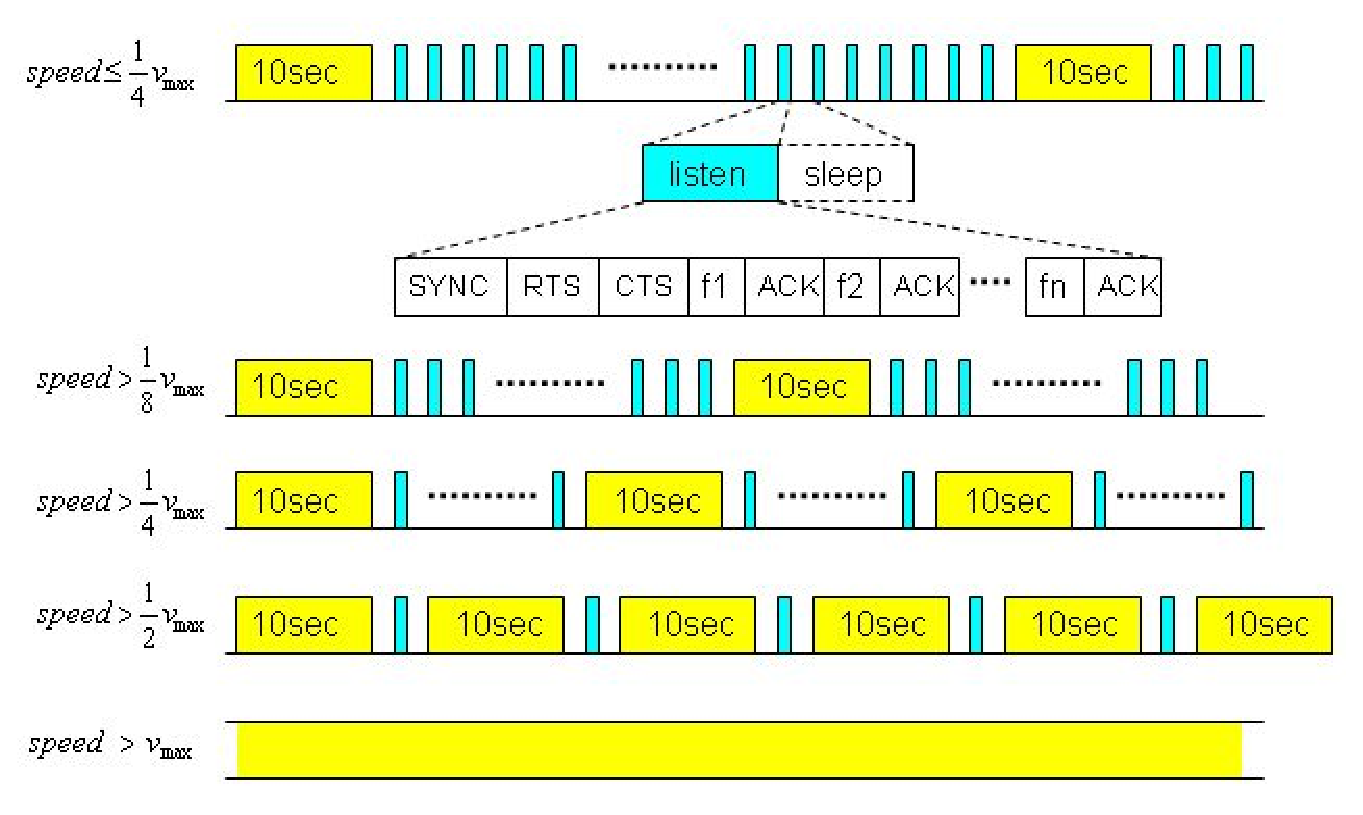
\includegraphics[scale=0.3, natwidth=0.38\textwidth]{msmac_timing}
		\caption{MS-MAC Timing Diagram}
	\label{fig:msmac-timing}
  \end{center}
\end{figure}



\subsubsection{MS-MAC}
%--- A para on current MAC protocol available. Classify them as Schedule based and contention based protocol. Why Schedule based protocol are better? Advantage of TDMA based protocols. --- \\ \\
 MS-MAC \cite{ms-mac} is a derivative of SMAC \cite{smac}, extended to support mobility. SMAC makes use of duty cycling to increase the sleep time of each node. This sleep/wake schedule is not global. In fact, SMAC organizes the network into virtual clusters, where nodes which possess a common schedule are grouped together as a cluster. The mobility information of each nodes is observed by the other nodes in the cluster. Based on the variation in the RSSI value of a mobile node, inter-cluster mobility of the node is detected by the cluster members. The cluster members then, form an active zone for a period of time, during with they adjust their synchronization frequency to support the mobile node in reaching the new cluster without losing connection to all its neighbours. \\\\

\begin{figure}[h]{} 
  \begin{center}
		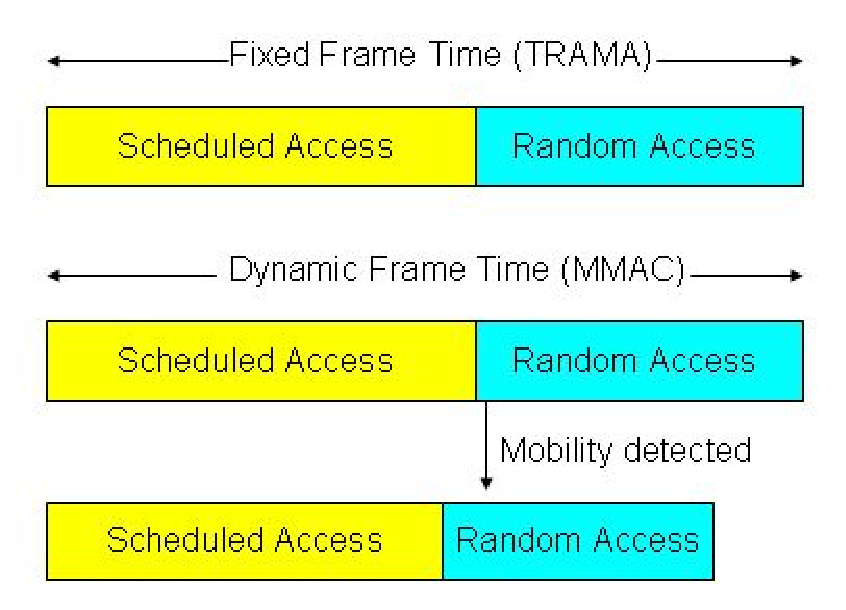
\includegraphics[scale=0.3, natwidth=0.38\textwidth]{mmac_timing}
		\caption{M-MAC Timing Diagram}
	\label{fig:mmac-timing}
  \end{center}
\end{figure}


\subsubsection{M-MAC}
M-MAC \cite{m-mac} is a scheduling based MAC protocol that employs a flexible frame time to adapt to mobility. Each round is divided into \emph{k} frames. During each frame, every node predicts its own location estimate for the next frame. This estimate is transmitted to the cluster head. The cluster head gathers the location information from each node, aggregates it and broadcasts it during the last slot of the current frame. This information provides the nodes in the cluster the knowledge of the mobility states of the cluster members, based on which a node chooses one of its neighbours to relay the data packets.

\begin{figure}[h]{} 
  \begin{center}
		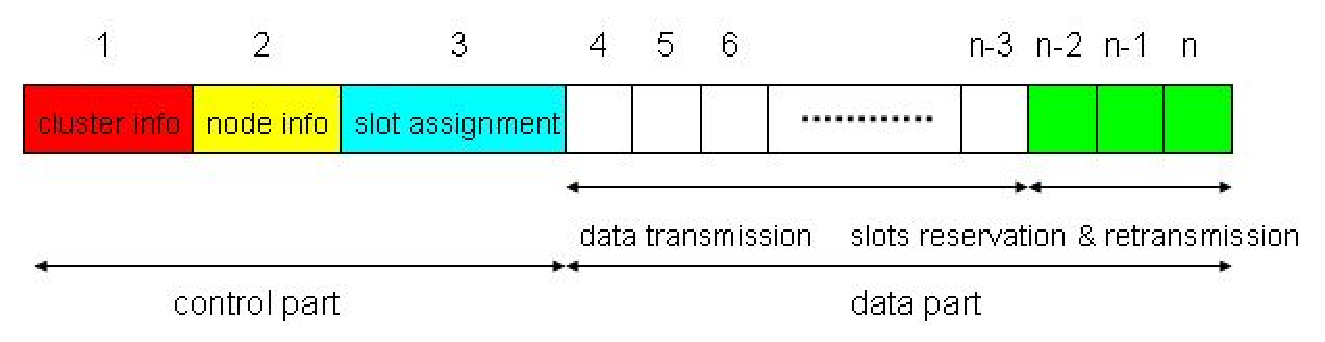
\includegraphics[scale=0.3, natwidth=0.38\textwidth]{mtdma_timing}
		\caption{M-TDMA: Timing Diagram}
	\label{fig:mtdma-timing}
  \end{center}
\end{figure}


\subsubsection{M-TDMA}
M-TDMA \cite{m-tdma} partitions the network into non-overlapping clusters based on FLOC algorithm\cite{floc}. Each cluster maintains a frame where a unique slot is provided for each cluster member. The slots are divided into control, data and reserved slots. The reserved slots are reserved for join requests from new nodes entering the cluster and message retransmissions. The control slots are divided to accomodate cluster information, node information and slot assignment. 

\begin{figure}[h]{} 
  \begin{center}
		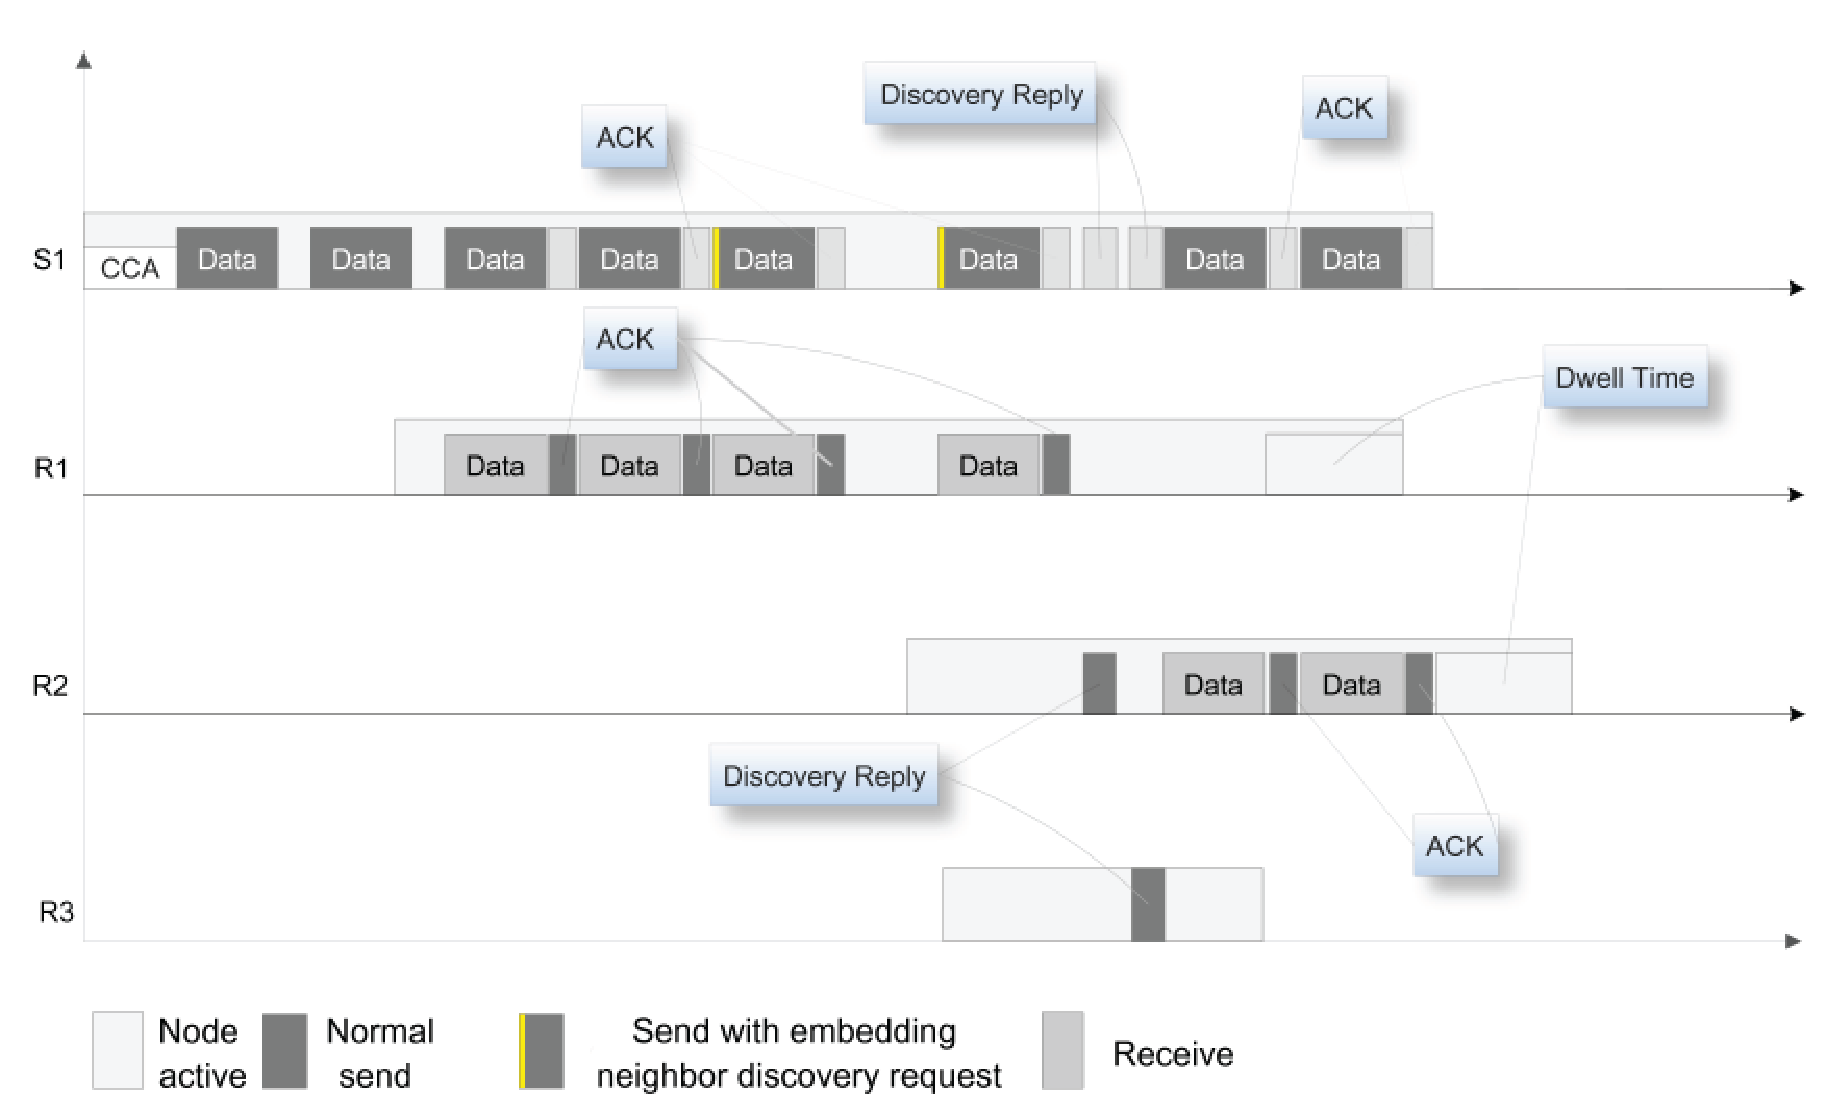
\includegraphics[scale=0.3, natwidth=0.38\textwidth]{mamac_timing}
		\caption{MA-MAC : Timing Diagram}
	\label{fig:mamac-timing}
  \end{center}
\end{figure}


\subsubsection{MA-MAC}
MA-MAC \cite{ma-mac} is a contention based protocol that primarily focusses on reliability of data transfer through seamless handover by adopting two distance thresholds. A sender \emph{$S_1$} initiates communication by transmitting a preamble packet to a receiver \emph{$R_1$}. When the receiver replies with an ACK message, the sender continues sending data packets. Over a period of time, the sender accumulates enough history RSSI values from the ACK packets sent by \emph{$R_1$}. At this point of time, it estimates its distance to the receiver. \emph{$S_1$} monitor this distance to see if it exceeds the distance threshold. When it exceeds the first threshold, \emph{$S_1$} starts embedding handover requests with the data packets, which it is broadcasting now. When another node \emph{$R_2$} receives this handover request, it replies with a handover reply. Now \emph{$S_1$} starts unicasting the data packets to \emph{$R_2$} instead of \emph{$R_1$}.  
 
\begin{figure}[h]{} 
  \begin{center}
		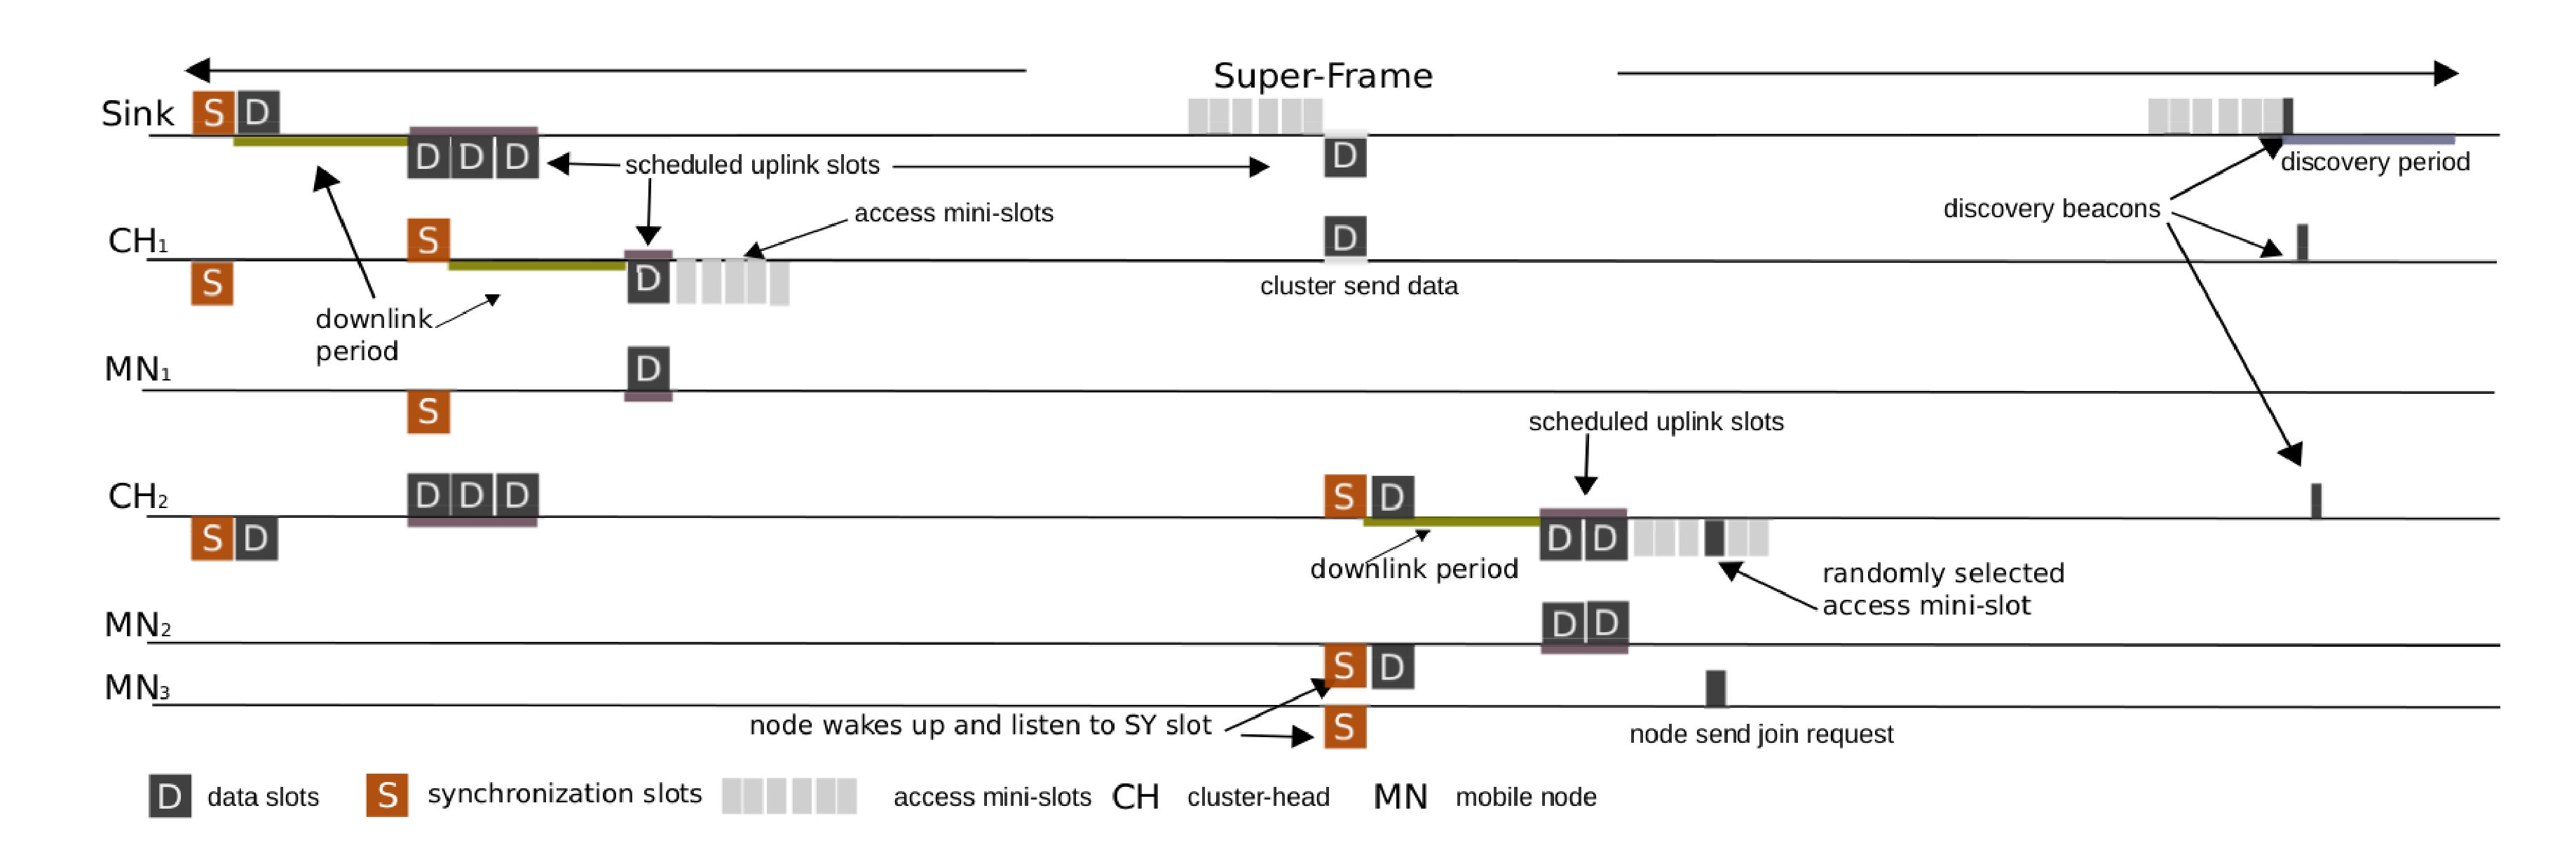
\includegraphics[scale=0.24, natwidth=0.38\textwidth]{mobisense_timing}
		\caption{Mobisense : Timing Diagram}
	\label{fig:mobisense-timing}
  \end{center}
\end{figure}


\subsubsection{Mobisense}
Mobisense \cite{mobisense} is a cross-layer architecture designed for micro-mobility scenarios. It assumes existence of a backbone static network which helps in routing data to the basestation. Each of the static nodes in the network act as a cluster head. Each cluster head operates in a different channel, maintains a cluster of mobile nodes, supports uplink and downlink transmission to and from the basestation. The super-frame is divided into Synchronization, Downlink and Uplink phase, access mini-slots and a discovery slot. During the discovery slot, the cluster head uses a common channel to  advertise information about the cluster. Any mobile node entering the cluster will collect information about the cluster and will send a join request during the access mini-slot. The cluster head adds the new mobile node to the cluster and adapts the schedule for downlink and uplink transmissions and broadcast the schedule information during the synchronization slot.  

\section{Opportunistic Routing}

Conventional routing techniques basically follow best-path routing, which assumes lossless communication links between nodes and a fixed topology. In an ideal wireless network with fixed channel conditions, best-path routing will provide excellant results. But this is not applicable to a Mobile Wireless Sensor network where due to the continuous movement of mobile nodes, the link quality between nodes and the overall topology of the network, continuously kepp changing. Best-path routing provides poor results in those channel conditions. As an alternative, Opportunistic routing gathers information about the current channel conditions and dynamically chooses a next-hop node based on the information. In the following sections we discuss three opportunisitc routing techniques: EXOR\cite{exor}, ROF\cite{rof} and OR-RSSI\cite{or-rssi}.  

\subsection{ROF: Receiver based Opportunistic Forwarding}
ROF is a Receiver-based forwarding technique which allows the receivers of the data packet to contend for forwarding rights before forwarding, instead of calculating and updating a routing path. This approach aims to solve three key problems in opportunistic routing: (i) Collision detection, (ii) Multicast suppression and (iii) Handling Routing voids, which are explained later in this section. The said problems are handled by using an optimized forwarding priority calculation and a dual-channel forwarding contention mechanism. It is assumed that each node in the network is location-aware. 

The first step in ROF is that the sender embeds its location in the data packet and broadcasts it. Each node receiving this packet is a potential forwarder. The receivers calculate a forwarding priority value considering their distance to sender and to that of base station, radio coverage radius and the remaining energy. If the distance between the receiver and the base station is higher than that of the sender and base station, the data packet is ignored. If not, then the receivers contend for forwarding rights in the contention window. The nodes contend by sending an ATF (Application To Forward) packet to the sender, at a particular slot in the contention window. The slot selection is based on the probability of sending ATF at each slot, which is a function of the priority value. 

The forwarding contention mechanism involves use of dual channels i.e. data and control channels. When the sender receives an ATF packet from one of the receiver, it is considered the winner of the forwarding rights and the sender immediately sends a busy tone on the control channel. To complement this process, each receiver after sending an ATF packet, listen to the control channel for a short period of time for a busy tone from the sender. If it hears a busy tone, it becomes aware that it has won the forwarding rights and stops contending immediately, and so does every other node. The use of dual-channel avoid the hidden terminal problem where a receiver node $N_j$, may not hear the ATF packet sent by Node $N_i$ to the sender and hence still contend for rights and sends its own ATF message to sender, causing the multicast problem. 

If collision of ATF packets occurs, the sender will be unable to decode the received message and hence decides that collision has occured. To manage this situation, the sender sends repetitive busy tone on the control channel. On hearing which, the nodes that have sent ATF will send the ATF packets with probability of 1 during the next slot of the contention window. In case the sender has not received any ATF packets for a pre-decided wait time, it assumes a routing void and goes into over-stepping mode. The over-stepping mode follows the same contention process, except that the forwarding priority calculation ignores the distance to base station factor, thus making all nodes receiving the data packet a potential forwarder. 


\subsection{OR-RSSI}
OR-RSSI is an opportunistic routing mechanism for Mobile Wireless Sensor Networks based on RSSI, specifically designed for network with sparse distribution of nodes. This approach calculates an opportunistic probability (OP) based on the RSSI value of beacons periodically sent by base station and the mobility vector(MV). The node with the highest OP wins the forwarding rights. The sink periodically broadcasts beacons with high transmission power. The nodes receiving the beacons, update their OP value based on the RSSI of the beacon. The OP value for node $i$ w.r.t sink $s$, with a mobility vector $\vec{mv_i}$, is calculated based on equation \ref{eqn:orrsi-eqn01}, where $c$ and $\alpha$ are constants. 

\begin{equation}
	OP_{is} \gets OP_{is} + \frac{1}{|RSSI|} \times \alpha + \vec{mv_i} \times c
	\label{eqn:orrsi-eqn01}
\end{equation}

$\alpha$ ia a factor which influences the OP value based on RSSI. Mobility vector is a simple model which represents the movement of the node $i$ w.r.t the sink. $\vec{mv_i} = 1$ if node $i$ is moving towards sink, $\vec{mv_i} = -1$ if it is moving away and $\vec{mv_i} = 0$ otherwise. The 


\begin{figure}[h]{} 
  \begin{center}
		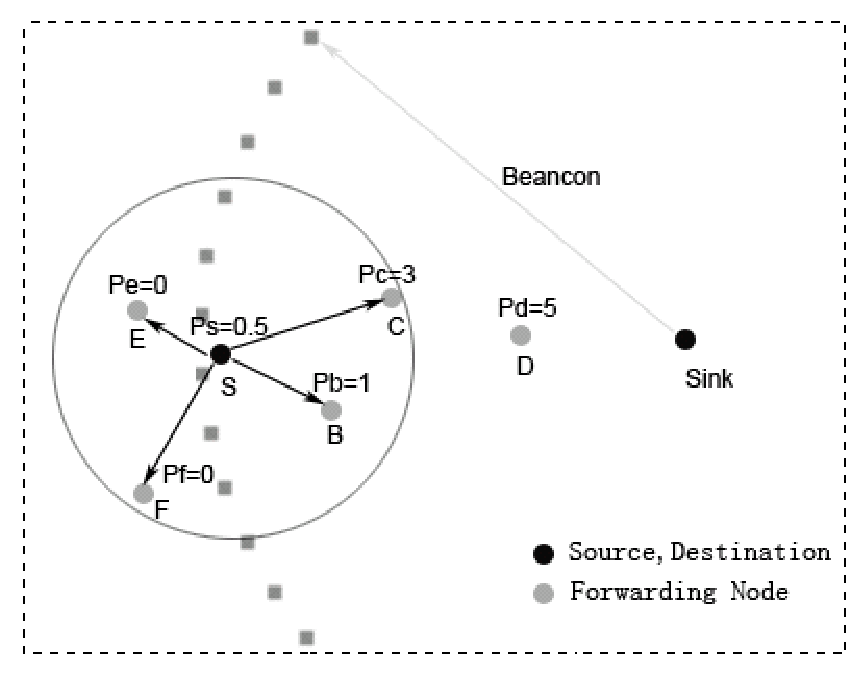
\includegraphics[scale=0.4, natwidth=0.38\textwidth]{orrssi_scenario01}
		\caption{OR-RSSI : Illustration}
	\label{fig:orrsssi-scenario}
  \end{center}
\end{figure}


\section{Time Synchronization}

\subsection{Need for Time Synchronization}
\subsection{Existing Techniques}
\subsubsection{RBS: Reference Broadcast Synchronization}
\subsubsection{TSPN: Timing-sync for sensor networks}
\subsubsection{FTSP: Flooding Time Synchronization Protocol}

\section{Mobility Estimation}
\subsection{Challenges}
\subsection{Techniques}





